\chapter{Background}
\label{cha:background}


\section{Word Embedding}
Recently machine learning algorithms are used often in many NLP tasks, but the machine can not directly understand human language. So the first thing is to transform the language to the mathematical form like word vectors, that is using digital vectors to represent words in natural languages. The above process is called word embedding. 

One of the easiest word embeddings is using a \emph{one-hot representation}, which uses a long vector to represent a word. It only has one component which is 1, and the other components are all 0s. The position of 1 corresponds to the index of the word in dictionary \gls{D}. But this word vector representation has some disadvantages, such as troubled by the huge dimensionality $|D|$. Most important it can not describe the similarity between words well. 

An alternative word embedding is the \emph{Distributed Representation}. It was firstly proposed by \cite{WilliamsHinton1986} and can overcome the above drawbacks from one-hot representation. The basic idea is to map each word into a short vector of fixed length (here \lq\lq short\rq\rq\ is with respect to \lq\lq long\rq\rq\  dimension $|D|$ of the one-hot representation). All of these vectors constitute a vector space, and each vector can be regarded as a point in the vector space. After introducing the \lq\lq distance\rq\rq in this space , it is possible to judge the similarity between words (morphology and syntax) according to the distance. 

There are many different models which can be used to estimate a Distributed Representation vector, including the famous LSA (Latent Semantic Analysis) \citep{DeerwesterDumaisEtAl1990} and the LDA (Latent Dirichlet Allocation) \citep{BleiNgEtAl2003}. In addition, the neural network algorithm based language model is a very common method and becomes more and more popular. A language model has the task to predict the next word in a sentence from the words observed so far.
In these neural network based models, the main goal is to generate a language model usually generating a word vectors as byproducts. In fact, in most cases, the word vector and the language model are bundled together. The first paper on this is the Neural Probabilistic Language Model from \citep{BengioDucharmeEtAl2003}, followed by a series of related research, including SENNA from \cite{CollobertWestonEtAl2011} and word2vec from  \cite{MikolovSutskeverEtAl2013}.

Word embedding actually is very useful. For example, Ronan Collobert's team makes use of the word vectors trained from software package SENNA (\citep{CollobertWestonEtAl2011}) to do part-of-speech tagging, chunking into phrases, named entity recognition and semantic role labeling, and achieves good results. 


\section{Neural Probabilistic Language Model}


\paragraph{Neural Network}\ 

General speaking, a neural network defines a mapping between some input and output, and it usually contains an input layer, an output layer and one or more hidden layers between the input layer and the output layer. Each layer has some nodes meaning that it can contains a vector with some dimension. Let $x(i-1)$ be the input vector to the $i$-th layer and $x(i)$ its output vector.
From one layer to the next layer, there is a map function $f(x(i-1))=x(i)$ made up by an \emph{activation function} with a weight matrix and and an offset vector. 

Specifically  vector $x(i-1)$ is  multiplied by a weight matrix $H$ and then adds an offset vector $q$, after that an activation function such as $tanh$ function shown as Figure \ref{fig:tanh}. Hence we have 
\begin{equation}
x(i) = f(x(i-1)) = \tanh(H * x(i-1)) + q
\end{equation}

\begin{figure}[tb]
  \centering
	\fbox{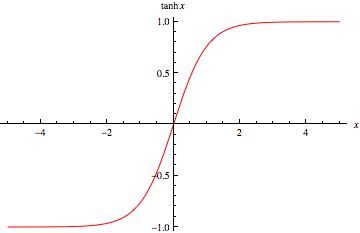
\includegraphics[width=0.4\textwidth]{tanh} }
	\caption{Graph of the $tanh$ function}
	\label{fig:tanh}
\end{figure}


Let's start with the simplest neural network with three layers (only one hidden layer) shown as Figure \ref{fig:neural3}. We can find that input layer has three nodes, that is the input should be a vector with dimension 3. The hidden layer has four nodes, which means the input vector will be mapped to a hidden vector with dimension 4. And then it will be mapped again to the output vector with dimension 2. Specifically, the input is a vector $x(0)$ (with dimension 3). $H$ (with size $4\times 3$) and $U$ (with size $2\times 4$) are respectively the weight matrix between input layer and hidden layer and the weight matrix between hidden layer and output layer, $p$ (with size 4) and $q$ (with size 2) are the offset vectors of respectively the hidden layer and the output layer. The activation function of the hidden layer is the $\tanh$ function 
and the activation function of the output layer is the identity function.  So we get the following formula
\begin{eqnarray}
x(1) &=&  \tanh(H * x(0)) + p, \qquad\qquad x(2) =  U * x(1) + q \nonumber \\
x(2) &=& U(\tanh(H * x(0)) + p) +q \label{eq:neural}
\end{eqnarray}


\begin{figure}[tb]
  \centering
	\fbox{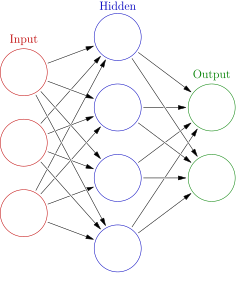
\includegraphics[width=0.4\textwidth]{neural3} }
	\caption{An example of neural network with three layers}
	\label{fig:neural3}
\end{figure}

\paragraph{Statistical Language Model}\ 

Statistical language models are widely used in natural language processing, speech recognition, machine translation. A Statistical language model is a probability model to calculate the probability of a sentence or word sequence, and is always built on a corpus \gls{C} containing sentences. 

Let $\gls{C}=(S_1,\ldots,S_M)$ be a corpus consisting of $M$ sentences $\gls{Si}=(w_{i,1},\ldots,w_{i,L_i})$, each of length $\gls{Li}$.  Then a language model computes the probability $p(C)$ of the corpus and the probabilities $p(S_i)$ of the sentences $S_i$ according to the conditional probability definition
\begin{eqnarray}
p(C) &=& \prod_{i = 1}^M p(S_i) \\
p(S_i)&=& \prod_{t=1}^{L_i} p(w_t|w_{t-1},\ldots,w_1)\nonumber \\
&\approx& \prod_{t=1}^{L_i} p(w_t|Prev(w_t)) \label{eq:languagemodel}
\end{eqnarray}
where $\gls{PrevNWt}=(w_{i,\max(t-n+1,1)},\ldots,w_{i,t})$ is the subsequence of $n-1$ past words before $w_t$ in sentence $S_i$. Note that the last equation is an approximation of the full conditional probability. The core part of a Statistic language model is to compute  $p(w_t|Prev(w_t))$ by some model if $Prev(w_t)$ is given.

\paragraph{Neural Probabilistic Language Model}\

\cite{BengioDucharmeEtAl2003} introduce a neural probabilistic language model shown as Figure \ref{fig:bengio}, which uses neural network to approximate $p(w_t|Prev(w_t))$
the language model (\ref{eq:languagemodel}).

\gls{C} is the given corpus containing the sentences/documents of words from a dictionary \gls{D}.
Consider a word $w_t$ in some sentence $S_i = (w_1,w_2,\ldots,w_{T-1},w_{L_i})$ of corpus \gls{C}, where $t$ is some position in $S$ and $L_i$ is the length of $S$. Let  $\gls{PrevNWt} = (w_{\max(t-n+1,1)},\ldots,w_{t-1})$ be the subsequence of words before $w_t$.  

Firstly for each word $w$ in dictionary \gls{D}, there is a look-up table $V$ mapping the word $w$ to vector $V(w)$. Note that $V$ is denoted as $C$ in figure \ref{fig:bengio}. The vector size of $V(w)$ is \gls{d}.
The input layer is a long vector concatenated by $n-1$ word vectors in $\gls{PrevNWt}$. So the input vector is $x$ with dimension $(n-1)d$, and the output vector is $y$ with the dimension |\gls{D}|, where \gls{D} is vocabulary and |\gls{D}| is the size of vocabulary.

\cite{BengioDucharmeEtAl2003} also use $\tanh$ function for the activation function in the hidden layer. $H$ (with size $m\times (n-1)d $) and $U$ (with size $|\gls{D}| \times m $) are respectively the weight matrix between input layer and hidden layer and the weight matrix between hidden layer and output layer, $p$ (with size $m$)and $q$ (with size $\gls{D}$) are the offset vectors of respectively the hidden layer and the output layer. Additionally, they introduce another weight matrix between the input layer and output layer $W$ (with size $|\gls{D}| \times (n-1)d$). So the mapping function from $x$ to the output is
\begin{equation}\label{eq:bengio}
y=q+U*\tanh(p+H*x) + W*x
\end{equation}

\begin{figure}[!ht]
  \centering
	\fbox{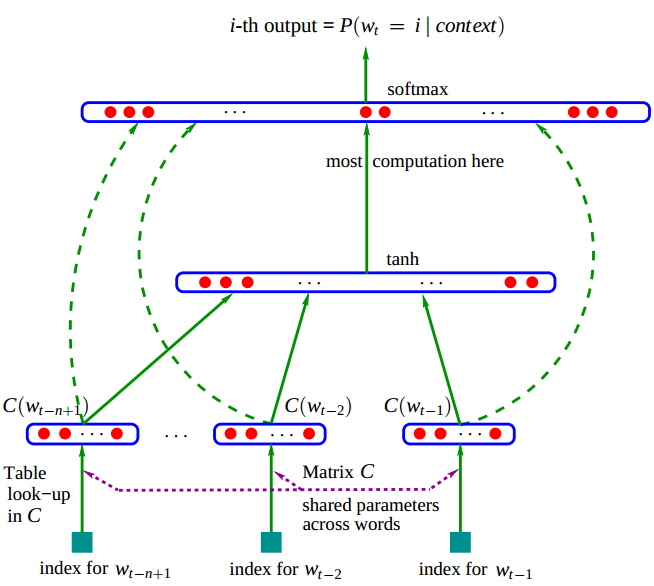
\includegraphics[width=0.7\textwidth]{bengio} }
	\caption{The neural network structure from \citep{BengioDucharmeEtAl2003}}
	\label{fig:bengio}
\end{figure}

\paragraph{Softmax Function}\ 

The softmax function, is a generalization of the logistic function that "squashes" a K-dimensional vector $z$ of arbitrary real values to a $K$-dimensional vector $\sigma(z)$ of real values in the range $(0,1)$ that add up to 1 \footnote{https://en.wikipedia.org/wiki/Softmax\_function}. The function is given by
$$\sigma(z)_j=\frac{e^{z_j}}{\sum^K_{k=1}e^{z_k}} \ \ \mathrm{for}\ j=1,\ldots,K.$$

From above, we know the output $y$ is a vector with the length of |\gls{D}| with arbitrary values and can not represent probabilities. Because it is a language model, it needs to model the probability as $p(w_t|Prev^{n-1}(w_t))$. Actually, \cite{BengioDucharmeEtAl2003} use the softmax function to do normalization. After normalization, the final result is a value between 0 to 1, which can represent a probability. Using $x_{w_t}$ to represent the input vector connected by word vectors from $Context(w_t)$ and $y_{w_t}$ to represent the output vector mapped from the neural network. From Formula \ref{eq:bengio} we have
\begin{equation}
y_{w_t}=q+U*\tanh(p+H*x_{w_t}) + W*x_{w_t}
\end{equation}
and $p(w_t|Prev^{n-1}(w_t))$ can be expressed as 
\begin{equation}\label{eq:softmax}
p(w_t|Prev^{n-1}(w_t))=\frac{e^{y_{w_t,i_{w_t}}}}{\sum^{|\gls{D}|}_{i=1}e^{y_{w_t,i}}},
\end{equation}
where $i_{w_t}$ represents the index of $w_t$ in the dictionary $D$, $y_{w_t,i}$ means the $i$-th element in the vector $y_{w_t}$. Note that the denominator contains a term $e^{y_{{w_t},i}}$ for every word in the vocabulary.
The goal is also to maximize the function shown as \ref{eq:languagemodel}. In the beginning, all word vectors are initialized randomly. And after maximizing the objective function, they can get the meaningful word vectors.

%--------------------------------------------------------------------------------------------------------------------------------%

\section{The model of Collobert and Weston}

The main purpose of the approach of \cite{CollobertWeston2008} originally is not to build a language model, but to use the word vectors from their model to complete several tasks from natural language processing, such as speech tagging, named entity recognition, phrase recognition, semantic role labeling, and so on (\citep{CollobertWeston2008} and \citep{CollobertWestonEtAl2011}). Due to the different purpose, their training method is also different. They do not use the Formula \ref{eq:languagemodel} as other language models used. Their idea is to optimize a score function on phrase so that if the phrase is reasonable or makes sense, the score would be positive, otherwise the score would be negative. 

\gls{C} is the given corpus with a vocabulary \gls{D} of size \gls{N}. Consider a word $w_t$ in some sentence $S = (w_1,w_2,\ldots,w_{T-1},w_{T})$ from corpus \gls{C}, where $t$ is some position of $S$ and $T$ is the length of $S$. Define $\gls{phraseWt} = (w_{t-c},\ldots,w_{t-1},w_t,w_{t+1},\ldots,w_{t+c})$, and $c$ is the number of words before and after $w_t$. Note that \gls{phraseWt} contains $w_t$. 
We define $phrase(w_t)^\prime$ as \gls{phraseWt} where the center word $w_t$ is replaced by  anther random word $w^\prime\not=w_t$. Each word is represented by a vector of dimension $d$ . For phrase \gls{phraseWt}, connect these $2c+1$ vectors to be a long vector $x_{w_t}$ with dimension $d \times (2c+1)$. The input of $f$ is the vector $x_{w_t}$ with dimension $d \times (2c+1)$. And the output is a real number (positive or negative). Use $x^\prime_{w_t}$ to represent the vector connected by $2c+1$ word vectors from $phrase(w_t)^\prime$.

\citep{CollobertWeston2008} also use a neural network to build their model. But the neural network structure is different from the network structure in \citep{BengioDucharmeEtAl2003}. Its output layer has only one node representing the score, rather than Bengio's \gls{N} nodes, where \gls{N} is the size of dictionary \gls{D}. Note that Bengio's model uses another softmax funtion to get the probability value in order to represent the Formula \ref{eq:softmax}. Doing so greatly reduced the computational complexity.

Based on the above description, the model use $f$ to represent its neural network, the input is a phrase vector, the output can be an arbitrary real number. Note that there is no active function in the output layer. The objective of this model is that for every phrase $phrase(w_t)$ from corpus,  $f(x_{w_t})$ should be always positive and $f(x^\prime_{w_t})$ should be always negative. Specifically the model gives an objective function to be minimized as following
\begin{equation}\label{eq:skipgram}
\sum_{w\in C}max\{0,1-f(x_{w}),f(x^\prime_{w})\}
\end{equation}
In most cases, replacing the middle of the word in a normal phrase, the new phrase is certainly not the normal phrase, which is a good method to build negative sample (in most cases they are negative samples, only in rare cases the normal phrases are considered as negative samples but they would not affect the final result). 


\section{Word2Vec}

The main purpose of Word2Vec is to accelerate the training process and simplify the model. 

Word2Vec actually contains two different models: the CBOW model (Continuous Bag-of-Words Model),   and the Skip-gram model(Continuous Skip-gram model), which uses the following objective function 
\begin{equation}
\prod_{w\in C}p(Context(w)|w),
\end{equation}
where $Context(w)$ are the words close to word $w$. Note that this criterion is related to but different from the language model criterion \ref{eq:languagemodel}.


Again \gls{C} is the given corpus with vocabulary \gls{D} containing  \gls{N} different words. Considering a word $w_t$ in some sentence $S = (w_1,w_2,\ldots,w_{T-1},w_{T})$ from corpus \gls{C}, where $t$ is some position of $S$ and $T$ is the length of $S$, they define\\
$\gls{contextWt} = (w_{,\max(t-c,1)},\ldots,w_{t-1},w_{t+1},\ldots,w_{,\min(t+c,T)})$, and $c$ is the number of words before and after $w_t$ in  $\gls{contextWt} $. The Figure \ref{fig:word2vec} shows the structures of CBOW model and Skip-gram model when $c=2$. 
\begin{figure}[!ht]
  \centering
	\fbox{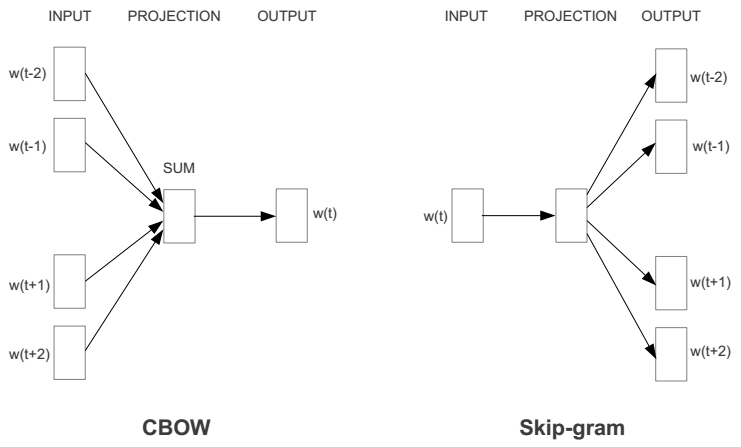
\includegraphics[width=0.9\textwidth]{word2vec} }
	\caption{word2vec}
	\label{fig:word2vec}
\end{figure}

In both neural networks from CBOW and Skip-gram model, the input is a vector with length $d$, for CBOW the input is the context vector calculated by average vector of words in the context, for the skip-gram model the input is the word vector of $w_t$. And the output is the vector of length $N$, (the size of the vocabulary). Obviously their prediction strategies are different. CBOW uses the context to predict the center word. And Skip-gram model uses the center word to predict the words in the context.  

\paragraph{Skip-gram model with negative sampling}\ 

Next we will focus on Skip-gram model with negative sampling to optimize the objective function  (\ref{eq:skipgram}). Let $V$ and $U$ represent  the set of input embedding vectors and the set of output embedding vectors respectively. And each embedding vectors has the dimension $d$. Additionally, $V_{w} \in \Re^d$ % V_{w,s}
means the input embedding vectors from word $w$. Similarly
$U_{w} \in \Re^d$ % U_{w,s} 
is the output embedding of word $w$ where  $w\in D$, $1\leq s\leq N_w$. The number of negative samples is \gls{K}. %$K$ 
And $P(w)$ is the smoothed unigram distribution which is used to generate negative samples. Specifically for each $w\in D$
$$P(w) = \frac{count(w)^{\frac{3}{4}}}{(\sum_{i=1}^M L_i)^{\frac{3}{4}}}$$ 
where $count(w)$ is the number of times $w$ occurred in $C$ and $\sum_{i=1}^M L_i$ is the number of total words in $C$. The objective function of skip-gram model with negative sampling can be defined specifically as

\begin{equation}
\begin{split}
G = \frac{1}{M}\sum_{i=1}^M\frac{1}{L_i}\sum_{t=1}^{L_i}\sum\limits_{\mbox{\tiny$\begin{array}{c}-c\leq j \leq c\\ j\neq 0\\ 1\leq j+t\leq L_i\end{array}$}}\Big \{\mathrm{log}\ p(w_{i,t+j}|w_{i,t}) 
+\sum\limits_{k=1}^K\mathbb{E}_{z_k\sim P(w)}\mathrm{log}\ [1-p(z_k|w_{i,t}) ] \Big \}
\end{split}
\end{equation} 

where $p(w^\prime|w) = \sigma({U_{w^\prime}}^{\mathrm{T}}V_w)$
 and $\sigma(x) = \frac{1}{1+\mathrm{e}^{-x}}$.\\
 
 $p(w_{i,t+j}|w_{i,t})$ is the probability of using center word $w_{i,t}$ to predict one surrounding word $w_{i,t+j}$, which needs to be \textbf{maximized}.
$z_1$,\ldots,$z_K$ are the negative sample words to replace word $w_{i,t+j}$, and $p(z_k|w_{i,t})\ (1\leq k\leq K)$ is the probability of using center word $w_{i,t}$ to predict one negative sample word $z_k$, which needs to be \textbf{minimized}. Equivalently, the whole objective function needs to be \textbf{maximized}. \\ 

Take the word pair $(w_{i,t},w_{i,t+j})$ as a training sample, and define \textbf{loss function} $loss$ for each sample 
\begin{eqnarray}
loss(w_{i,t},w_{i,t+j})
 &=& -\mathrm{log}\ p(w_{i,t+j}|w_{i,t})-\sum\limits_{k=1}^K\mathbb{E}_{z_k\sim P(w)}\mathrm{log}\ [1-p(z_k|w_{i,t})] 
\end{eqnarray}
Here the loss is defined as the negative log probability of $w_{i,t}$ given $w_{i,t+j}$. 

And the loss function of whole corpus is $$loss(C)=\frac{1}{M}\sum_{i=1}^M\frac{1}{L_i}\sum_{t=1}^{L_i}\sum\limits_{\mbox{\tiny$\begin{array}{c}-c\leq j \leq c\\ j\neq 0\\ 1\leq j+t\leq L_i\end{array}$}}loss(w_{i,t},w_{i,t+j})$$
To maximize the objective function is equivalently to minimize the loss function. So the objective of learning algorithm is 
$$\arg\min_{\{V,U\}} \frac{1}{M}\sum_{i=1}^M\frac{1}{L_i}\sum_{t=1}^{L_i}\sum\limits_{\mbox{\tiny$\begin{array}{c}-c\leq j \leq c\\ j\neq 0\\ 1\leq j+t\leq L_i\end{array}$}}loss(w_{i,t},w_{i,t+j})$$ 

Use 
$$It = \frac{1}{M}\sum_{i=1}^M\frac{1}{L_i}\sum_{t=1}^{L_i}\sum\limits_{\mbox{\tiny$\begin{array}{c}-c\leq j \leq c\\ j\neq 0\\ 1\leq j+t\leq L_i\end{array}$}} 1$$
to represent the number of total training samples in one epoch. (An epoch is a measure of the number of times all of the training samples are used once.) And the number of epochs is $T$. So the total iterations is $It*T$.\\
	
Use stochastic gradient descent:\footnote{https://en.wikipedia.org/wiki/Stochastic\_gradient\_descent} 
	\begin{itemize}
	\item Initialize $\{V,U\}$
	\item For $It*T$ Iterations: 
		\begin{itemize}
		\item For each training sample $(w_{i,t},w_{i,{t+j}})$
		\begin{itemize}
		\item Generate negative sample words to replace $w_{i,t+j}$: $(w_1,\ldots,z_k)$
		\item Calculate the gradient $\Delta = -\nabla_{\{V,U\}} loss(w_{i,t},w_{i,{t+j}})$
		\item $\Delta$ is only made up by $\{\Delta_{V_{w_{i,t}}}, \Delta_{U_{w_{i,t+j}}}, [\Delta_{U_{w_1}},\ldots,\Delta_{U_{z_k}}]\}$
		\item Update Embeddings: 
		\begin{itemize}
		\item $V_{w_{i,t}} = V_{w_{i,t}}+\alpha\Delta_{V_{w_{i,t}}}$
		\item $U_{w_{i,t+j}} = U_{w_{i,t+j}}+\alpha\Delta_{U_{w_{i,t+j}}}$
		\item $U_{z_k} = U_{z_k}+\alpha\Delta_{U_{z_k}}, 1\leq k\leq K$ 
		\end{itemize}
		($\alpha$ is the learning rate and will be updated every several iterations)
		\end{itemize}
		\end{itemize}
	\end{itemize}
The detail of gradient calculation of $loss(w_{i,t},w_{i,t+j})$ is
\begin{eqnarray*}
	\Delta_{V_{w_{i,t}}} &=& -\frac{\partial loss(w_{i,t},w_{i,t+j})}{\partial V_{w_{i,t}}} = [1-\mathrm{log}\ \sigma(U_{w_{i,t+j}}^{\mathrm{T}}V_{w_{i,t}})]U_{w_{i,t+j}}+\sum_{i=1}^k [-\mathrm{log}\ \sigma(U_{z_k}^{\mathrm{T}}V_{w_{i,t}}))]U_{z_k}\\
	\Delta_{U_{w_{i,t+j}}} &=& -\frac{\partial loss(w_{i,t},w_{i,t+j})}{\partial U_{w_{i,t+j}}} = [1-\mathrm{log}\ \sigma(U_{w_{i,t+j}}^{\mathrm{T}}V_{w_{i,t}})]V_{w_{i,t}}\\
	\Delta_{U_{z_k}} &=& -\frac{\partial loss(w_{i,t},w_{i,t+j})}{\partial U_{z_k}} = [-\mathrm{log}\ \sigma(U_{z_k}^{\mathrm{T}}V_{w_{i,t}}))]V_{w_{i,t}}, 1\leq k\leq K
\end{eqnarray*}
